\documentclass[12pt,a4paper]{article}

% ─── Page Layout ───────────────────────────────────────────────────────────────
\usepackage[a4paper, margin=0.8in, headheight=14pt]{geometry}

% ─── Fonts (XeLaTeX) ───────────────────────────────────────────────────────────
\usepackage{fontspec}
\usepackage{unicode-math}
\setmainfont{TeX Gyre Pagella}
\setmonofont[Scale=0.88]{TeX Gyre Cursor}
\setmathfont{Latin Modern Math}

% ─── Packages ──────────────────────────────────────────────────────────────────
\usepackage{xcolor}
\usepackage{colortbl}
\usepackage{titlesec}
\usepackage{enumitem}
\usepackage{tabularx}
\usepackage{booktabs}
\usepackage{array}
\usepackage{amsmath}
\usepackage{tikz}
\usetikzlibrary{shapes.geometric, arrows.meta, positioning, calc, fit, decorations.pathreplacing, patterns}
\usepackage{tcolorbox}
\tcbuselibrary{skins, breakable}
\usepackage{hyperref}
\usepackage{fancyhdr}
\usepackage{graphicx}
\usepackage{microtype}
\hyphenpenalty=10000
\exhyphenpenalty=10000
\sloppy
\usepackage{caption}
\usepackage{setspace}
\usepackage{multirow}
\usepackage{tocloft}

% ─── Q&A helper ────────────────────────────────────────────────────────────────
\newcommand{\Q}[1]{\textbf{#1}\par\noindent\ignorespaces}

% ─── Colour Palette ────────────────────────────────────────────────────────────
\definecolor{myred}{RGB}{196,30,58}
\definecolor{mydark}{RGB}{30,30,50}
\definecolor{mygreen}{RGB}{14,120,80}
\definecolor{myteal}{RGB}{0,130,140}
\definecolor{myamber}{RGB}{180,100,0}
\definecolor{mypurple}{RGB}{100,30,160}
\definecolor{mygray}{RGB}{246,247,249}
\definecolor{mgframe}{RGB}{180,185,200}
\definecolor{watermark}{RGB}{145,150,170}
\definecolor{hdrred}{RGB}{250,232,235}
\definecolor{hdrgreen}{RGB}{220,244,233}
\definecolor{hdrteal}{RGB}{220,242,244}
\definecolor{hdramber}{RGB}{253,242,215}
\definecolor{hdrpurple}{RGB}{238,228,255}
\definecolor{hdrgray}{RGB}{238,240,245}
\definecolor{rowalt}{RGB}{250,251,253}

% ─── Section Formatting ────────────────────────────────────────────────────────
\titleformat{\section}
  {\large\bfseries\color{myred}}{\thesection.}{0.5em}{}
  [\vspace{1pt}{\color{myred}\rule{\linewidth}{0.8pt}}]
\titleformat{\subsection}
  {\normalsize\bfseries\color{myteal}}{\thesubsection}{0.5em}{}
\titlespacing*{\section}{0pt}{18pt}{7pt}
\titlespacing*{\subsection}{0pt}{11pt}{4pt}

% ─── Paragraph ─────────────────────────────────────────────────────────────────
\setlength{\parindent}{0pt}
\setlength{\parskip}{4pt}

% ─── TOC Styling ───────────────────────────────────────────────────────────────
\renewcommand{\cfttoctitlefont}{\large\bfseries\color{myred}}
\renewcommand{\cftaftertoctitle}{\par\noindent{\color{myred}\rule{\linewidth}{0.8pt}}}
\setlength{\cftbeforetoctitleskip}{0pt}
\setlength{\cftaftertoctitleskip}{6pt}
\renewcommand{\cftsecfont}{\normalsize\bfseries\color{mydark}}
\renewcommand{\cftsecpagefont}{\normalsize\bfseries\color{mydark}}
\renewcommand{\cftsecleader}{\cftdotfill{\cftdotsep}}
\setlength{\cftbeforesecskip}{7pt}
\renewcommand{\cftsubsecfont}{\small\color{mydark}}
\renewcommand{\cftsubsecpagefont}{\small\color{mydark}}
\setlength{\cftbeforesubsecskip}{3pt}
\setlength{\cftsubsecindent}{1.4em}

% ─── Table helpers ─────────────────────────────────────────────────────────────
\renewcommand{\arraystretch}{1.45}
\setlength{\tabcolsep}{6pt}
\arrayrulecolor{mydark}
\newcolumntype{B}[1]{>{\small\bfseries\raggedright\arraybackslash}m{#1}}
\newcolumntype{Y}{>{\small\raggedright\arraybackslash}X}
\renewcommand{\tabularxcolumn}[1]{m{#1}}

% ─── Header / Footer ───────────────────────────────────────────────────────────
\pagestyle{fancy}
\fancyhf{}
\fancyhead[L]{\small\color{myred}\textbf{26-ES-EE101}\;\color{mydark}--- Basic Electrical and Electronics Engineering}
\fancyhead[R]{\small\color{myteal}\textbf{Module 3 Notes}}
\fancyfoot[C]{\small\color{mydark}\thepage}
\fancyfoot[R]{\small\color{watermark}\textit{\copyright\ Biraj}}
\renewcommand{\headrulewidth}{0.5pt}
\renewcommand{\footrulewidth}{0.3pt}

% ─── Hyperref ──────────────────────────────────────────────────────────────────
\hypersetup{
  colorlinks=true, linkcolor=myteal, urlcolor=myteal,
  pdfauthor={Biraj Sarkar (CGEC)},
  pdftitle={26-ES-EE101 --- Module 3 Notes: Alternating-Current Circuits}
}

% ─── tcolorbox styles ──────────────────────────────────────────────────────────
\tcbset{
  tikzbox/.style={
    colback=mygray, colframe=mgframe, boxrule=0.6pt, arc=4pt,
    left=8pt, right=8pt, top=6pt, bottom=6pt,
    colbacktitle=mgframe, coltitle=mydark, fonttitle=\small\bfseries
  },
  defbox/.style={
    colback=hdrgreen, colframe=mygreen, boxrule=0.8pt, arc=4pt,
    left=9pt, right=9pt, top=6pt, bottom=6pt,
    colbacktitle=mygreen, coltitle=white, fonttitle=\small\bfseries
  },
  formulabox/.style={
    colback=hdrteal, colframe=myteal, boxrule=0.8pt, arc=4pt,
    left=9pt, right=9pt, top=7pt, bottom=7pt,
    colbacktitle=myteal, coltitle=white, fonttitle=\small\bfseries
  },
  examplebox/.style={
    colback=hdramber, colframe=myamber, boxrule=0.8pt, arc=4pt,
    left=9pt, right=9pt, top=6pt, bottom=6pt,
    colbacktitle=myamber, coltitle=white, fonttitle=\small\bfseries
  },
  masonbox/.style={
    colback=hdrpurple, colframe=mypurple, boxrule=0.8pt, arc=4pt,
    left=9pt, right=9pt, top=6pt, bottom=6pt,
    colbacktitle=mypurple, coltitle=white, fonttitle=\small\bfseries
  },
  exambox/.style={
    colback=hdrpurple, colframe=mypurple, boxrule=1pt, arc=5pt,
    left=10pt, right=10pt, top=8pt, bottom=8pt,
    colbacktitle=mypurple, coltitle=white, fonttitle=\bfseries,
    breakable, title after break={\textbf{Frequently Asked / Viva Questions (contd.)}}
  }
}
\tcbset{breakable}
\tcbset{after={\par\color{black}}}

% ─── TikZ styles ───────────────────────────────────────────────────────────────
\tikzset{
  block/.style={rectangle, draw=myteal, fill=hdrteal,
    text width=2.4cm, align=center, minimum height=0.95cm,
    font=\small, rounded corners=3pt, line width=0.7pt},
  redblock/.style={rectangle, draw=myred, fill=hdrred,
    text width=2.4cm, align=center, minimum height=0.95cm,
    font=\small, rounded corners=3pt, line width=0.7pt},
  sumjunc/.style={circle, draw=myamber, fill=hdramber,
    minimum size=0.62cm, font=\small, line width=0.8pt},
  arrow/.style={-Stealth, thick, color=mydark},
  redarrow/.style={-Stealth, thick, color=myred},
  line/.style={thick, color=mydark}
}

\begin{document}

% ─── Title Page ───────────────────────────────────────────────────────────────
\begin{center}
  {\Large\bfseries\color{myred} 26-ES-EE101}\\[3pt]
  {\LARGE\bfseries\color{myred} Basic Electrical and Electronics Engineering}\\[5pt]
  {\normalsize\color{mydark} Semester I \quad$\bullet$\quad 3L:1T:0P \quad$\bullet$\quad 4 Credits}\\[3pt]
  {\normalsize\color{myteal}\textbf{Module 3 Exam Notes: Alternating-Current Circuits}}\\[3pt]
  {\small\color{mydark} CGEC \;$|$\; MAKAUT Syllabus (A.Y. 2026--27) \;$|$\; \textit{Biraj Sarkar}}
\end{center}
\vspace{2pt}
\noindent{\color{myred}\rule{\linewidth}{1.5pt}}
\vspace{2pt}

\hypersetup{linkcolor=mydark}
\tableofcontents
\hypersetup{linkcolor=myteal}
\newpage

\section{Alternating-Current Circuits}

\subsection{Generation and measurement of AC}
\begin{tcolorbox}[defbox,title={Alternating voltage, period and RMS value}]
An alternating voltage changes polarity periodically. Its period \(T\) is the time for one cycle. Its root-mean-square (RMS) value equals the DC voltage that delivers the same average power to a given resistor.
\end{tcolorbox}

For \(N\) turns, uniform field \(B\) and coil area \(A\), the angle from the field to the coil normal is \(\omega t\). The flux per turn is \(BA\cos\omega t\). With the reference polarity set by Faraday's law,
\[
\begin{aligned}
v(t)&=-N\frac{d}{dt}(BA\cos\omega t)\\
    &=NBA\omega\sin\omega t
     =V_m\sin\omega t,\\
\omega&=2\pi f,\qquad T=\frac{1}{f}.
\end{aligned}
\]
Here \(f\) is in Hz, \(\omega\) in rad/s and \(V_m\) is the peak in volts. The signed cycle average of this sinusoid is zero. In form-factor calculations, use the average of the rectified waveform:
\[
\begin{aligned}
V_{\mathrm{av,rect}}
 &=\frac{1}{\pi}\int_0^\pi V_m\sin\theta\,d\theta
 =\frac{2V_m}{\pi},\\
V_{\mathrm{rms}}
 &=\sqrt{\frac{1}{2\pi}\int_0^{2\pi}V_m^2\sin^2\theta\,d\theta}
 =\frac{V_m}{\sqrt2},\\
\text{form factor}
 &=\frac{V_{\mathrm{rms}}}{V_{\mathrm{av,rect}}}=\frac{\pi}{2\sqrt2}\approx1.111,\\
\text{peak factor}
 &=\frac{V_m}{V_{\mathrm{rms}}}=\sqrt2.
\end{aligned}
\]
Use \(\sin^2\theta=(1-\cos2\theta)/2\) to evaluate the RMS integral. Apply the same definitions to current.

\subsection{Phasors and RLC circuits}
A phasor is a complex number representing the RMS magnitude and phase of a sinusoid at a fixed frequency. With cosine reference, \(v(t)=\sqrt2 V\cos(\omega t+\theta)\) corresponds to \(\underline V=V\angle\theta\). Compare phases only after expressing all quantities with the same frequency and sine or cosine reference.

\begin{itemize}[leftmargin=*, itemsep=3pt, topsep=4pt]
  \item \textbf{Impedance and admittance.} \(Z=\underline V/\underline I=R+jX\) is in \(\Omega\). \(Y=1/Z=G+jB_s\) is in S, with \(B_s\) the susceptance.
  \item \textbf{Resistor.} \(Z_R=R\). Current and voltage are in phase.
  \item \textbf{Inductor.} The derivative in \(v_L=L\,di_L/dt\) becomes \(j\omega\), so \(Z_L=j\omega L\). Current lags voltage by \(90^\circ\).
  \item \textbf{Capacitor.} From \(i_C=C\,dv_C/dt\), \(Z_C=1/(j\omega C)\). Current leads voltage by \(90^\circ\).
\end{itemize}

Add impedances in series and admittances in parallel:
\[
\begin{aligned}
Z_{\mathrm{series}}&=R+j\left(\omega L-\frac{1}{\omega C}\right),\\
Y_{\mathrm{parallel}}&=\frac{1}{R}
       +j\left(\omega C-\frac{1}{\omega L}\right).
\end{aligned}
\]
\begin{itemize}[leftmargin=*, itemsep=3pt, topsep=4pt]
  \item \textbf{Parallel branches.} The displayed expression assumes separate ideal \(R,L,C\) branches. In general, use \(Y_{\mathrm{in}}=\sum_k 1/Z_k\), then \(\underline I=\underline VY_{\mathrm{in}}\).
  \item \textbf{Series phasors.} With current as reference, \(V_R\) lies on the real axis, \(V_L\) points up and \(V_C\) points down. The net reactive voltage is \(I(X_L-X_C)\).
\end{itemize}

\begin{tcolorbox}[tikzbox,title={Series RLC phasors for a net inductive load},unbreakable]
\centering
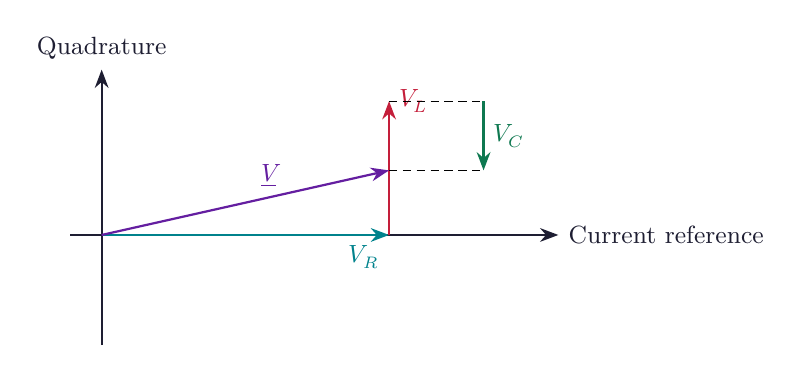
\begin{tikzpicture}[font=\small]
\draw[arrow] (-0.4,0)--(5.8,0) node[right] {Current reference};
\draw[arrow] (0,-1.4)--(0,2.1) node[above] {Quadrature};
\draw[arrow,myteal] (0,0)--(3.65,0) node[below left] {$V_R$};
\draw[arrow,myred] (3.65,0)--(3.65,1.7) node[right] {$V_L$};
\draw[arrow,mygreen] (4.85,1.7)--(4.85,0.82) node[midway,right] {$V_C$};
\draw[densely dashed] (3.65,1.7)--(4.85,1.7) (3.65,0.82)--(4.85,0.82);
\draw[arrow,mypurple] (0,0)--(3.65,0.82) node[pos=0.58,above] {$\underline V$};
\end{tikzpicture}
\end{tcolorbox}

\begin{tcolorbox}[examplebox,title={Solving a series RLC circuit}]
Apply \(100\angle0^\circ\,\mathrm V\) RMS to \(R=30\,\Omega\), \(X_L=60\,\Omega\), \(X_C=20\,\Omega\).
\[
\begin{aligned}
Z&=30+j40=50\angle53.13^\circ\,\Omega,\\
\underline I&=\frac{100\angle0^\circ}{50\angle53.13^\circ}\\
             &=2\angle(-53.13^\circ)\,\mathrm A.
\end{aligned}
\]
The lagging power factor is \(30/50=0.60\). The component voltage magnitudes are \(60\), \(120\) and \(40\,\mathrm V\). Their phasor sum has magnitude \(\sqrt{60^2+(120-40)^2}=100\,\mathrm V\).
\end{tcolorbox}

\begin{tcolorbox}[examplebox,title={Find the input of a parallel RLC circuit}]
For \(100\angle0^\circ\,\mathrm V\) RMS across separate \(R=50\,\Omega\), \(X_L=100\,\Omega\) and \(X_C=50\,\Omega\) branches,
\[
\begin{aligned}
Y&=\frac{1}{50}-j\frac{1}{100}+j\frac{1}{50}
  =0.020+j0.010\,\mathrm S,\\
\underline I&=100Y=2+j1\,\mathrm A,\\
Z&=\frac{1}{Y}=40-j20\,\Omega.
\end{aligned}
\]
Current leads voltage because the net susceptance is positive. The current magnitude is \(\sqrt5\,\mathrm A\).
\end{tcolorbox}

\subsection{Power and power-factor improvement}
\begin{tcolorbox}[defbox,title={Active, reactive and apparent power}]
Active power \(P\) is average energy delivered per second (W). Reactive power \(Q\) measures the quadrature part of the power exchange (var). Apparent power \(S\) is the product of RMS voltage and current (VA).
\end{tcolorbox}

Let \(\phi=\angle\underline V-\angle\underline I\). The product of the instantaneous sinusoids is \(VI[\cos\phi+\cos(2\omega t-\phi)]\) when \(v(t)=\sqrt2V\cos\omega t\). The double-frequency term averages to zero. Thus
\[
\begin{aligned}
\underline S&=\underline V\underline I^*=P+jQ,\\
P&=VI\cos\phi,& Q&=VI\sin\phi,\\
S&=VI=\sqrt{P^2+Q^2},& \mathrm{PF}&=P/S.
\end{aligned}
\]
Here \(Q>0\) for a net inductive load and \(Q<0\) for a net capacitive load. For sinusoidal passive loads the displacement power factor is \(\cos\phi\). In the series example \(P=120\,\mathrm W\), \(Q=160\,\mathrm{var}\), \(S=200\,\mathrm{VA}\).

\textbf{Procedure for correcting a lagging power factor.}
\begin{enumerate}[leftmargin=*, itemsep=3pt, topsep=4pt]
  \item Find the reactive demand before and after correction using \(Q=P\tan\phi\). Use the same active power \(P\).
  \item Select a shunt capacitor to supply \(Q_C=P(\tan\phi_1-\tan\phi_2)\), the difference between the old and target demands.
  \item For a single-phase supply, use \(C=Q_C/(\omega V^2)\) with RMS voltage \(V\). The supply current falls at the same active power because the source supplies less reactive current.
\end{enumerate}
At \(50\,\mathrm{Hz}\), cancelling the earlier \(160\,\mathrm{var}\) at \(100\,\mathrm V\) requires
\[
\begin{aligned}
C&=\frac{160}{2\pi(50)(100)^2}\,\mathrm F\\
 &=50.9\,\mu\mathrm F .
\end{aligned}
\]
In the ideal example supply current falls from \(2\,\mathrm A\) to \(1.2\,\mathrm A\); load-branch current is still \(2\,\mathrm A\).

\subsection{Series and parallel resonance}
Resonance means cancellation of the input reactive term at a particular frequency. In series RLC set \(X_L=X_C\). For parallel RLC with ideal reactive branches set their susceptances to cancel.
\[
\begin{aligned}
\omega_0 L &=\frac{1}{\omega_0 C},\\
f_0 &=\frac{1}{2\pi\sqrt{LC}}.
\end{aligned}
\]
\begin{itemize}[leftmargin=*, itemsep=3pt, topsep=4pt]
  \item \textbf{Series.} \(Z=R\) is minimum and the supply current is maximum at fixed voltage. The individual reactive voltages can be large. Quality factor is \(\omega_0L/R\).
  \item \textbf{Parallel.} With ideal \(L,C\) and \(R\) in separate branches, \(Y=1/R\) is minimum and supply current is minimum. The reactive branch currents can still be large. Coil resistance shifts the resonant frequency.
  \item \textbf{Numerical check.} \(L=0.1\,\mathrm H\) and \(C=100\,\mu\mathrm F\) give \(f_0\approx50.3\,\mathrm{Hz}\) in the ideal model.
\end{itemize}

\subsection{Balanced three-phase systems}
A balanced source has equal sinusoidal phase voltages spaced by \(120^\circ\). A balanced load presents equal phase impedances. In star, one end of each phase connects to the neutral point. The line voltage is the difference of two phase voltages. For a positive sequence,
\[
\begin{aligned}
\underline V_{AB}
 &= V_{\mathrm{ph}}\angle0^\circ-V_{\mathrm{ph}}\angle(-120^\circ)\\
 &=\sqrt3 V_{\mathrm{ph}}\angle30^\circ .
\end{aligned}
\]
Line current equals phase current in star. In delta the phases form a closed triangle so \(V_L=V_{\mathrm{ph}}\). A line current is a difference of two branch currents, for example \(\underline I_A=\underline I_{AB}-\underline I_{CA}\), so \(I_L=\sqrt3 I_{\mathrm{ph}}\) for a balanced delta.

\begin{tcolorbox}[formulabox,title={Balanced three-phase power}]
\[
\begin{aligned}
P_3&=3V_{\mathrm{ph}}I_{\mathrm{ph}}\cos\phi
    =\sqrt3 V_L I_L\cos\phi,\\
Q_3&=\sqrt3 V_L I_L\sin\phi,\qquad
S_3=\sqrt3 V_L I_L .
\end{aligned}
\]
\end{tcolorbox}

\textbf{Three-phase power measurement.}
For a three-wire load, place wattmeter current coils in lines A and B and use C as the common voltage-coil return. The meters sense \(V_{AC}\) with \(I_A\), and \(V_{BC}\) with \(I_B\). Since \(i_A+i_B+i_C=0\), the sum of the instantaneous meter products is
\[
(v_A-v_C)i_A+(v_B-v_C)i_B=v_Ai_A+v_Bi_B+v_Ci_C.
\]
The average therefore gives \(P_3=W_1+W_2\), including algebraic signs. In a balanced load, with the meters labelled so that \(W_1=V_L I_L\cos(30^\circ-\phi)\) and \(W_2=V_L I_L\cos(30^\circ+\phi)\),
\[
\tan\phi=\sqrt3\frac{W_1-W_2}{W_1+W_2}.
\]
A lagging angle above \(60^\circ\) gives a negative \(W_2\) in this labelling. In a four-wire load, one wattmeter per phase can give the total by summation. 
\begin{tcolorbox}[examplebox,title={Balanced star load and wattmeter readings}]
Take \(V_L=400\,\mathrm V\) and \(Z_{\mathrm{ph}}=20\angle36.87^\circ\,\Omega\).
\[
\begin{aligned}
V_{\mathrm{ph}}&=\frac{400}{\sqrt3}=230.94\,\mathrm V,\\
I_L&=I_{\mathrm{ph}}=\frac{230.94}{20}=11.55\,\mathrm A,\\
P_3&=\sqrt3(400)(11.547)(0.80)\approx6.40\,\mathrm{kW}.
\end{aligned}
\]
The meters read approximately \(4.59\,\mathrm{kW}\) and \(1.81\,\mathrm{kW}\). Their sum agrees with \(P_3\).
\end{tcolorbox}

\newpage
\begin{center}
  {\large\bfseries\color{myred} Quick Revision --- Module 3}\\[3pt]
  {\small\color{mydark} Alternating-Current Circuits $|$ 26-ES-EE101}
\end{center}
\noindent{\color{myred}\rule{\linewidth}{1.2pt}}
\vspace{4pt}

\begin{tcolorbox}[formulabox, title={Key Formulas and Concepts at a Glance}]
\renewcommand{\arraystretch}{1.35}
\begin{tabularx}{\linewidth}{B{4.4cm}Y}
Sinusoidal RMS and mean & $V_{\mathrm{rms}}=V_m/\sqrt2$; $V_{\mathrm{av,rect}}=2V_m/\pi$. \\[3pt]
Complex power & $\underline S=\underline V\underline I^*=P+jQ$. \\[3pt]
Resonance & $f_0=1/(2\pi\sqrt{LC})$ for the ideal models. \\[3pt]
Balanced AC power & $P_3=\sqrt3 V_L I_L\cos\phi$. \\[3pt]
\end{tabularx}
\end{tcolorbox}

\begin{tcolorbox}[defbox, title={One-Line Definitions}]
\textbf{Impedance.} Complex voltage-to-current ratio at a stated frequency.

\textbf{Power factor.} Ratio of active power to apparent power.

\textbf{Resonance.} Condition in which input reactance or susceptance cancels at a particular frequency.
\end{tcolorbox}

\begin{tcolorbox}[exambox, title={Frequently Asked / Viva Questions}]
\begin{enumerate}[topsep=0pt, label=\textbf{Q\arabic*.}, itemsep=5pt]
  \item \Q{Why is a sinusoid's cycle average zero?} Its equal positive and negative half cycles cancel.
  \item \Q{Which average is used in form factor?} Average of the rectified waveform.
  \item \Q{What is an RMS phasor?} An RMS amplitude with a phase reference for one sinusoidal frequency.
  \item \Q{Which way does inductor current shift?} It lags the voltage by $90^\circ$ for an ideal inductor.
  \item \Q{Why add admittances for parallel branches?} Each branch has common voltage and branch currents add.
  \item \Q{What is the sign of Q for a capacitor?} Negative with the passive load convention.
  \item \Q{Why use a shunt capacitor with inductive loads?} It reduces reactive power drawn from the supply.
  \item \Q{When is series current highest?} At resonance for a fixed sinusoidal supply voltage.
  \item \Q{How do line and phase voltages relate in star?} $V_L=\sqrt3 V_{\mathrm{ph}}$ in a balanced system.
  \item \Q{How are the two wattmeter readings used?} Add their signed values for total active power.
\end{enumerate}
\end{tcolorbox}

\begin{tcolorbox}[tikzbox, title={Summary Reference}]
\begin{tabularx}{\linewidth}{|B{4.0cm}|Y|}\hline
Topic & \textbf{What to remember} \\ \hline
R, L and C & Current phase relative to voltage is $0^\circ$, $-90^\circ$ and $+90^\circ$ respectively. \\ \hline
Series versus parallel resonance & Compare maximum and minimum supply current. \\ \hline
Star versus delta & Star shares a neutral point. Delta joins the phases in a closed loop. \\ \hline
\end{tabularx}
\end{tcolorbox}

\end{document}

